\documentclass[10pt]{article} %tipo documento y tipo letra

\definecolor{azulc}{cmyk}{0.72,0.58,0.42,0.20} % color titulo
\definecolor{naranja}{cmyk}{0.21,0.5,1,0.03} % color leccion

\def\eje{\centerline{\textbf{ EJERCICIOS.}}} % definiciones propias

\begin{document}

\begin{quote}

% inicio encabezado
{\color{gray}
\begin{tabular}{@{\extracolsep{\fill}}lcr}
\docLink{../cap3/geometria23.tex}{\includegraphics{../../images/navegacion/anterior.gif}}
\begin{tabular}{l}
{\color{darkgray}\small Cap. 3. Volumen} \\ \\ \\
\end{tabular} &
\docLink[_top]{../../index.html}{\includegraphics{../../images/navegacion/inicio.gif}}
\docLink{../../docs_curso/contenido.html}{\includegraphics{../../images/navegacion/contenido.gif}}
\docLink{../../docs_curso/descripcion.html}{\includegraphics{../../images/navegacion/descripcion.gif}}
\docLink{../../docs_curso/profesor.html}{\includegraphics{../../images/navegacion/profesor.gif}}
& \begin{tabular}{r}
{\color{darkgray}\small F�rmula Distancia} \\ \\ \\
\end{tabular}
\docLink{04_02.tex}{\includegraphics{../../images/navegacion/siguiente.gif}}
\\ \hline
\end{tabular}
}
%fin encabezado

%nombre capitulo
\begin{center}
\colorbox{azulc}{{\color{white} \large CAP�TULO 4}}  {\large
{\color{ azulc} FUNCIONES}}
\end{center}

\newline

%nombre leccion

\colorbox{naranja}{{\color{white} \normalsize  Lecci\'on 4.1. }}
{\normalsize {\color{naranja} El Plano Cartesiano}}

\newline

As� como a cada n�mero real se asigna un punto de una recta y
rec�procamente, a un punto de la recta se asigna un n�mero real, a
una pareja ordenada $(a,b)$ de n�meros reales se hace corresponder
un punto del plano y a cada punto del plano una pareja ordenada,
de la manera que veremos enseguida: se establece un {\bf sistema
de coordenadas rectangulares o cartesianas} en un plano dibujando
dos rectas coordenadas perpendiculares, una horizontal y una
vertical llamadas {\bf ejes coordenados}. Su punto de corte,
llamado {\bf origen del sistema} es denotado por 0. La recta
horizontal es el {\bf eje} $\mathbf{X}$ o eje de las $x$ o
abscisas y la vertical es el {\bf eje} $\mathbf {Y}$, eje de las
$y$ u ordenadas. La mitad positiva del eje $X$ se extiende hacia
la derecha y la mitad positiva del eje $Y$ se extiende hacia
arriba. Los ejes dividen el plano en cuatro partes llamadas
primero, segundo, tercero y cuarto {\bf cuadrantes}, usualmente
se�alados con I, II, III y IV. Los puntos de los ejes no est�n en
cuadrante alguno.

\newline

\begin{center}
\includegraphics{imagenes/a1.gif}
\end{center}

\newline

Dado un punto $P$ del plano, una recta vertical que pase por $P$,
corta el eje el $X$ en un punto $a$ y una recta horizontal que
pase por $P$, corta el eje $Y$ en un punto $b$. Al punto $P$ se le
asocia la pareja ordenada $(a,b)$. $a$ es llamada la {\bf
coordenada $x$ o abscisa de $P$} y $b$ {\bf la coordenada $y$ u
ordenada de $P$}. Se dice que $P$ tiene coordenadas $(a,b)$ y se
escribe $P(a,b)$. Rec�procamente, para una pareja ordenada $(a,b)$
de n�meros reales cualesquiera, tenemos que la recta vertical que
corta el eje $X$ en $a$ y la recta horizontal que corta el eje $Y$
en $b$ se intersectan en un punto $P$. Este se asocia a la pareja.
Las coordenadas de $ P$ son $(a,b)$.

\newline

\begin{center}
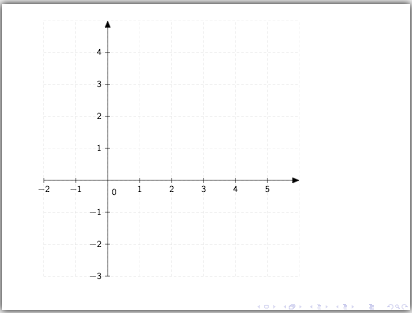
\includegraphics{imagenes/b1.gif}
\end{center}


%Pie de p�gina
\newline

{\color{gray}
\begin{tabular}{@{\extracolsep{\fill}}lcr}
\hline \\
\docLink{../cap3/geometria23.tex}{\includegraphics{../../images/navegacion/anterior.gif}}
\begin{tabular}{l}
{\color{darkgray}\small Cap. 3. Volumen} \\ \\ \\
\end{tabular} &
\docLink[_top]{../../index.html}{\includegraphics{../../images/navegacion/inicio.gif}}
\docLink{../../docs_curso/contenido.html}{\includegraphics{../../images/navegacion/contenido.gif}}
\docLink{../../docs_curso/descripcion.html}{\includegraphics{../../images/navegacion/descripcion.gif}}
\docLink{../../docs_curso/profesor.html}{\includegraphics{../../images/navegacion/profesor.gif}}
& \begin{tabular}{r}
{\color{darkgray}\small F�rmula Distancia} \\ \\ \\
\end{tabular}
\docLink{04_02.tex}{\includegraphics{../../images/navegacion/siguiente.gif}}
\end{tabular}
}

\end{quote}

\newline

\begin{flushright}
\includegraphics{../../images/interfaz/copyright.gif}
\end{flushright}
\end{document}
